%%%%%%%%%%%%%%%%%%%%%%%%%%%%%%%%%%%%%%%%%%%%%%%%
% Corrigé UPSTI
% Concours - Epreuve - Année
%%%%%%%%%%%%%%%%%%%%%%%%%%%%%%%%%%%%%%%%%%%%%%%%
\documentclass[11pt]{article}

%%%%%%%%%%%%%%%%%%%%%%%%%%%%%%%%%%%%%%%%%%%%%%%%
% Package UPSTI_Document
%%%%%%%%%%%%%%%%%%%%%%%%%%%%%%%%%%%%%%%%%%%%%%%% 
\usepackage{UPSTI_Corrige_Concours}	% Squelette minimal
%\usepackage[UPSTI]{UPSTI_Corrige_Concours} % Chargement des packages UPSTI  (téléchargeables ici: https://www.upsti.fr/documents-pedagogiques/upsti-kit-de-demarrage-latex)

%---------------------------------%
% Packages personnalisés
%---------------------------------%
% Insérez ici les packages que vous utilisez habituellement

%%%%%%%%%%%%
% Définition des vecteurs 
%%%%%%%%%%%%
\newcommand{\vect}[1]{\overrightarrow{#1}}
\newcommand{\axe}[2]{\left(#1,\vect{#2}\right)}
\newcommand{\couple}[2]{\left(#1,\vect{#2}\right)}
\newcommand{\angl}[2]{\left(\vect{#1},\vect{#2}\right)}

\newcommand{\rep}[1]{\mathcal{R}_{#1}}
\newcommand{\quadruplet}[4]{\left(#1;#2,#3,#4 \right)}
\newcommand{\repere}[4]{\left(#1;\vect{#2},\vect{#3},\vect{#4} \right)}
\newcommand{\base}[3]{\left(\vect{#1},\vect{#2},\vect{#3} \right)}


\newcommand{\vx}[1]{\vect{x_{#1}}}
\newcommand{\vy}[1]{\vect{y_{#1}}}
\newcommand{\vz}[1]{\vect{z_{#1}}}

% d droit pour le calcul différentiel
\newcommand{\dd}{\text{d}}

\newcommand{\inertie}[2]{I\left({#1}, #2\right)}
\newcommand{\matinertie}[7]{
\begin{pmatrix}
#1 & #6 & #5 \\
#6 & #2 & #4 \\
#5 & #4 & #3 \\
\end{pmatrix}_{#7}}
%%%%%%%%%%%%
% Définition des torseurs 
%%%%%%%%%%%%

\newcommand{\ec}[2]{%
\mathcal{E}_{c\;\left(#1/#2\right)}}

\newcommand{\pext}[3]{%
\mathcal{P}_{\left(#1\rightarrow#2/#3\right)}}

\newcommand{\pint}[3]{%
\mathcal{P}_{\left(#1 \stackrel{\text{#3}}{\leftrightarrow} #2\right)}}


 \newcommand{\torseur}[1]{%
\left\{{#1}\right\}
}

\newcommand{\torseurcin}[3]{%
\left\{\mathcal{#1} \left(#2/#3 \right) \right\}
}

\newcommand{\torseurci}[2]{%
\left\{\sigma \left(#1/#2 \right) \right\}
}
\newcommand{\torseurdyn}[2]{%
\left\{\mathcal{D} \left(#1/#2 \right) \right\}
}


\newcommand{\torseurstat}[3]{%
\left\{\mathcal{#1} \left(#2\rightarrow #3 \right) \right\}
}


 \newcommand{\torseurc}[8]{%
%\left\{#1 \right\}=
\left\{
{#1}
\right\}
 = 
\left\{%
\begin{array}{cc}%
{#2} & {#5}\\%
{#3} & {#6}\\%
{#4} & {#7}\\%
\end{array}%
\right\}_{#8}%
}

 \newcommand{\torseurcol}[7]{
\left\{%
\begin{array}{cc}%
{#1} & {#4}\\%
{#2} & {#5}\\%
{#3} & {#6}\\%
\end{array}%
\right\}_{#7}%
}

 \newcommand{\torseurl}[3]{%
%\left\{\mathcal{#1}\right\}_{#2}=%
\left\{%
\begin{array}{l}%
{#1} \\%
{#2} %
\end{array}%
\right\}_{#3}%
}

% Vecteur vitesse
 \newcommand{\vectv}[3]{%
\vect{V_{{#2}/{#3}}}\left( {#1}\right)
}

% Vecteur force
\newcommand{\vectf}[2]{%
\vect{R_{ {#1} \rightarrow {#2}}}
}

% Vecteur moment stat
\newcommand{\vectm}[3]{%
\vect{\mathcal{M}_{{#2} \rightarrow {#3}}}    \left( {#1}\right)
}




% Vecteur résultante cin
\newcommand{\vectrc}[2]{%
\vect{R_{c\;{{#1}/ {#2}}}}
}
% Vecteur moment cin
\newcommand{\vectmc}[3]{%
\vect{\sigma_{{#2}/{#3}}}\left( {#1}\right)
}


% Vecteur résultante dyn
\newcommand{\vectrd}[2]{%
\vect{R_{d\;{{#1}/ {#2}}}}
}
% Vecteur moment dyn
\newcommand{\vectmd}[3]{%
\vect{\delta_{{#2}/{#3}}}\left( {#1}\right)
}

% Vecteur accélération
 \newcommand{\vectg}[3]{%
\vect{\Gamma_{{#2}/{#3}}}\left( {#1}\right)
}

% Vecteur omega
 \newcommand{\vecto}[2]{%
\vect{\Omega_{{#1}/{#2}}}
}
% }$$\left\{\mathcal{#1} \right\}_{#2} =%
% \left\{%
% \begin{array}{c}%
%  #3 \\%
%  #4 %
% \end{array}%
% \right\}_{#5}}
\usepackage{amsmath}

\usepackage{siunitx}
\sisetup{output-decimal-marker = {,}}

% ---

%---------------------------------%
% Paramètres du corrigé
%---------------------------------%

% ----------
% Concours
% ----------
% 0: Custom*
% 1: ATS
% 2: Banque PT
% 3: CCINP
% 4: CCP
% 5: CCS (par défaut)
% 6: E3A
% 7: ICNA
% 8: Mines AADN
% 9: Mines Ponts
% 10: X-ENS
% * Si on met la valeur 0, il faut décommenter la ligne suivante: 		
%\newcommand{\UPSTIconcoursCustom}{Concours custom}
\newcommand{\UPSTIidConcours}{5}

% ----------
% Filière
% ----------
% 0: Custom*
% 1: ATS
% 2: MP
% 3: MPI
% 4: PSI (par défaut)
% 5: PT
% 6: TSI
% 7: MP2I
% 8: MPSI
% 9: PCSI
% 10: PTSI
% * Si on met la valeur 0, il faut décommenter la ligne suivante: 		
%\newcommand{\UPSTIfiliereCustom}{Filière custom}
\newcommand{\UPSTIidFiliere}{4}

% ----------
% Epreuve
% ----------
% 0: Custom*
% 1: S2I (par défaut)
% 2: Informatique
% 3: Modélisation et informatique
% 4: Modélisation
% 5: Physique - SI
% 6: SI A
% 7: SI B
% 8: SI C
% 9: SI 1
% 10: SI 2
% * Si on met la valeur 0, il faut décommenter la ligne suivante: 		
%\newcommand{\UPSTIepreuveCustom}{Epreuve custom}
\newcommand{\UPSTIidEpreuve}{1}

% ----------
% Session
% ----------
\newcommand{\UPSTIsession}{2020}

% ----------
% Titre de l'épreuve (souvent, le nom du support)
% ----------
\newcommand{\UPSTItitreEpreuve}{Robotisation du désherbage mécanique des vignes}
% Si le nom est trop long pour l'entête, on peu décommenter la ligne suivante:
\newcommand{\UPSTItitreEpreuveRaccourci}{Robot Bakus}      

%----------------------------------------------- 
\UPSTIprepareDocument		% "Compile" les variables
%%%%%%%%%%%%%%%%%%%%%%%%%%%%%%%%%%%%%%%%%%%%%%%% 


%%%%%%%%%%%%%%%%%%%%%%%%%%%%%%%%%%%%%%%%%%%%%%%% 
% Début du document
%%%%%%%%%%%%%%%%%%%%%%%%%%%%%%%%%%%%%%%%%%%%%%%% 
\begin{document}
\UPSTIpreambuleEpreuve	% Affichage du préambule de l'épreuve

%---------------------------------%
% DEBUT du contenu
%---------------------------------%

%\UPSTItitrePartieCorrige{Titre de la partie}


\begin{center}
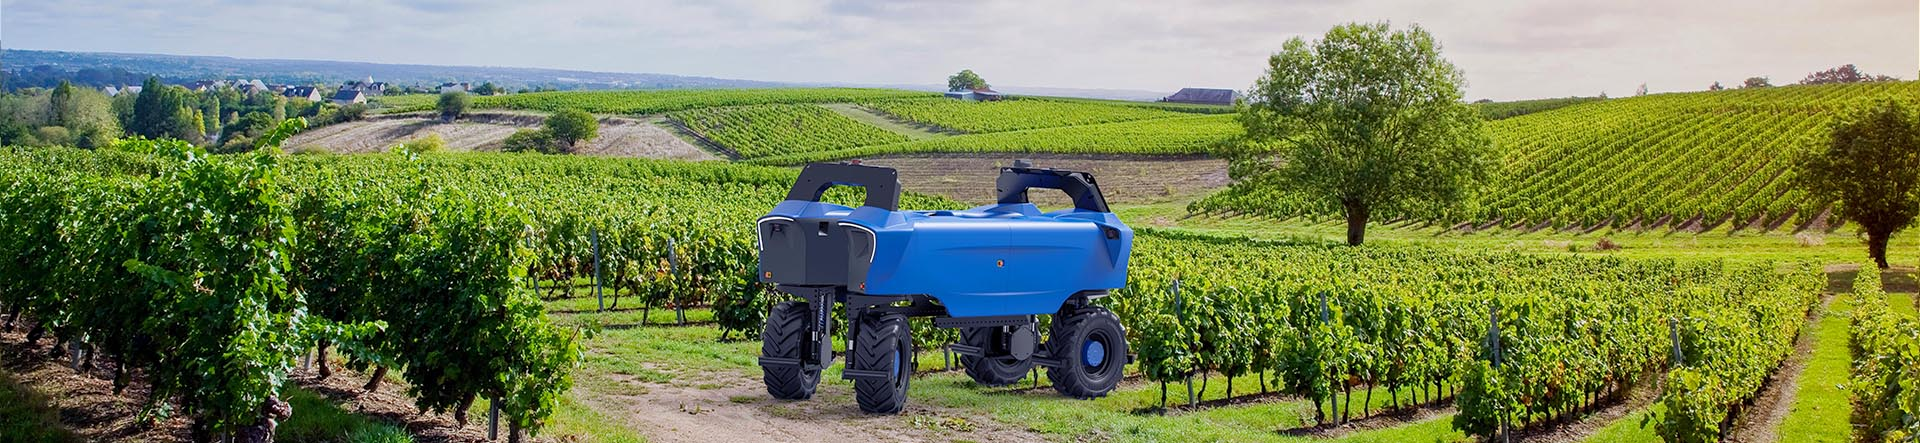
\includegraphics[width=\linewidth]{images/bakus-vigne}

\footnotesize \url{https://vitibot.fr/img/bakus-vigne.jpg}
\normalsize
\end{center}
\section{Génération des consignes d'orientation des roues avant et arrière pour le guidage du robot Bakus}

\UPSTIobjectif{
Élaborer les lois permettant de générer les consignes d'orientation à envoyer à chacune des quatre roues orientables du robot, afin qu'il puisse se déplacer le long d'un rang de vigne avec la même précision qu'un tracteur piloté par un chauffeur.
}

\subsection{Changement de variables $\left (y_{G_2},\theta \right) \rightarrow \left(y_F,y_R\right)$}

% -------------------------- 
% Boite d'objectif 
% -------------------------- 
\UPSTIobjectif{
Simplifier l'approche du problème d'asservissement du couple de variables $\left (y_{G_2},\theta \right)$ au point de fonctionnement $\left(0,0\right)$ à l'aide d'un changement de variables approprié.
}
% -------------------------- 

%\subsubsection{Test subsubsection}

% -------------------------- 
% Question (sans le saut de ligne qui la précède par défaut) + corrigé
% -------------------------- 
%\UPSTIquestion* Question (sans ligne vide, car à la suite d'un titre) On utilise la commande étoilée UPSTIquestion*

\UPSTIquestion* À partir de la figure A uniquement : 
\begin{itemize}
\item déterminer les expressions linéarisées à l'ordre 1 de $y_F$ et $y_R$, notées respectivement (E1) et (E2) en fonction de $y_{G_2}$, $\theta$ et $L$ puis en déduire l'expression de $\theta$ en fonction de $y_F$, $y_R$ et $L$ notée (E3);
\item déduire de ces résultats que chercher à asservir le couple de variables $\left (y_{G_2},\theta \right)$ au point de fonctionnement $\left(0,0\right)$  est équivalent à asservir $\left(y_F,y_R\right)$ au même point de fonctionnement.
\end{itemize}

\begin{UPSTIcorrige}

\textbf{Expression (E1)}

En se plaçant dans le quadrilatère $F F_0 G_0 G_2$, on a $\vect{F F_0} + \vect{F_0 G_0}+\vect{G_0 G_2}+\vect{G_2 F}=\vect{0}$. 

Tout d'abord, on a $\vect{G_0 F_0} = L\cos \theta \vect{x_0}$. On a alors : $y_F \vect{y_0} - L\cos \theta \vect{x_0} - y_{G_2} \vect{y_0} + L\vect{x_2}=\vect{0}$.  

On demande d'exprimer $y_F$; donc on projette cette expression suivant  $\vect{y_0}$. On obtient donc 
$y_F - y_{G_2}  + L\vect{x_2}\cdot \vect{y_0}=0$ soit $y_F - y_{G_2}  + L\sin \theta=0$ et   $y_F - y_{G_2}  + L \theta=0$  (E1).

\textbf{Expression (E2)}

En se plaçant dans le quadrilatère $G_2 G_0 R_0 R$, on a $\vect{G_2 G_0} + \vect{ G_0 R_0}+\vect{R_0 R}+\vect{R G_2 }=\vect{0}$. 

On a de même $\vect{R_0 G_0} = L\cos \theta \vect{x_0}$. On a alors : $y_{G_2} \vect{y_0} - L\cos \theta \vect{x_0} - y_{R} \vect{y_0} + L\vect{x_2}=\vect{0}$.  

On demande d'exprimer $y_R$; donc on projette cette expression suivant  $\vect{y_0}$. On obtient donc 
$y_{G_2}  - y_{R}  + L\vect{x_2}\cdot \vect{y_0}=0$ soit $y_{G_2}  - y_{R}  + L\sin \theta=0$ et $y_{G_2}  - y_{R}  + L \theta=0$ (E2).

Ou alors par définition :

\begin{itemize}
\item $y_F=\vect{OF}\cdot \vect{y}_0=\left(\vect{OG_2}+\vect{G_2F}\right)\cdot \vect{y}_0$.

On obtient alors : 

$y_F=y_{G_2}+L\vect{x}_2\cdot \vect{y}_0=y_{G_2}+L\sin\theta$ (E1)

\item $y_R=\vect{OR}\cdot \vect{y}_0=\left(\vect{OG_2}+\vect{G_2R}\right)\cdot \vect{y}_0$.

On obtient alors : 

$y_R=y_{G_2}-L\vect{x}_2\cdot \vect{y}_0=y_{G_2}-L\sin\theta$ (E2)
\end{itemize} 




\textbf{Expression (E3)}

On a d'une part $y_{G_2} = y_F  + L \theta$  (E1) et d'autre part $y_{G_2}  = y_{R}  - L \theta$ (E2).
En conséquence,  $y_F  + L \theta =  y_{R}  - L \theta$  soit $  \theta = \dfrac{ y_{R} - y_F}{2L } $ (E3).



\textbf{Bilan}

Autour du point de fonctionnement en linéarisant les relations géométriques on obtient un système linéaire de deux équations. On a alors 2 relations indépendantes (E1) et (E2) pour 4 paramètres. Il y a donc deux mobilités. On peut donc choisir de piloter ou d'imposer deux couples paramètres au choix par exemple  $\left (y_{G_2},\theta \right)$ ou $\left(y_F,y_R\right)$.

Au point de fonctionnement $\left(0,0\right)$, piloter un couple de variables $\left (y_{G_2},\theta \right)$ permet de piloter de façon unique un couple $\left(y_F,y_R\right)$. Réciproquement, piloter un couple de variables $\left(y_F,y_R\right)$ permet de piloter de façon unique un couple $\left (y_{G_2},\theta \right)$ --  \textit{CQFD}.

\end{UPSTIcorrige}


\subsection{Modélisation cinématique étendue du robot}


\UPSTIobjectif{
Établir un modèle exploitable décrivant les déplacements du robot Bakus sur le sol naturel, c'est-à-dire en tenant compte d'un éventuel glissement des roues sur le sol lorsqu'il est en dévers (phénomène de dérive latérale et angulaire). 
}

\subsubsection{Notations et hypothèses}

\subsubsection{Mise en équation du modèle cinématique étendu du robot Bakus}

\UPSTIquestion* À partir de la figure A, déterminer les relations donnant les expressions de :
\begin{itemize}
\item $\dot{y}_F$ et $\dot{y_R}$ en fonction de $V_F$, $V_R$, $\theta$, $\delta_F$, $\delta_R$, $\beta_F$ et $\beta_R$;
\item $\dot{x}_{G_2}$ en fonction de $V_{G_2}$, $\gamma_{G_2}$ et $\theta$.
\end{itemize}

\begin{UPSTIcorrige}

\begin{center}
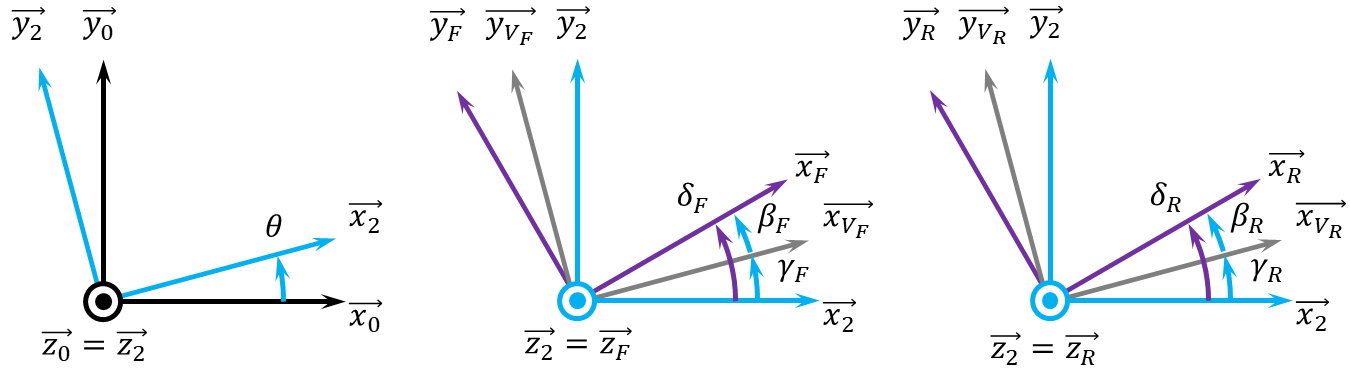
\includegraphics[width=.75\linewidth]{images/fig_01}
\end{center}
\textbf{Expression de $\dot{y}_F$}

On a  $\vectv{F}{2}{0}=\vect{V}_F = \dot{x}_F \vect{x_0} +\dot{y}_F \vect{y_0}$ (problème plan).  
Par ailleurs, en projetant $\vect{V}_F $ dans la base $\mathcal{B}_0$, on a $\vect{V}_F =V_F\vect{x_{V_F}}$ 
$=V_F\left(\cos\left(\gamma_F +\theta \right)\vect{x_0}+\sin\left(\gamma_F +\theta \right)\vect{y_0}\right)$. Enfin, $\delta_F=\gamma_F+\beta_F$ $\Leftrightarrow \gamma_F = \delta_F-\beta_F  $. 
En projetant  $\vectv{F}{2}{0}$ sur $\vect{y_0}$ on a $V_F\sin\left(\delta_F-\beta_F +\theta \right) = \dot{y}_F $.

\textbf{Expression de $\dot{y}_R$}

De manière analogue, on a $V_R \sin\left(\delta_R-\beta_R +\theta \right) = \dot{y}_R $.

\textbf{Expression de $\dot{x}_{G_2}$}

On a  $\vectv{G_2}{2}{0}=\vect{V}_G = \dot{x}_{G_2} \vect{x_0} +\dot{y}_{G_2} \vect{y_0}$.  
Par ailleurs, en projetant $\vect{V}_{G_2} $ dans la base $\mathcal{B}_0$, on a $\vect{V}_{G_2} =V_{G_2}\vect{x_{V_{G_2}}}$ 
$=V_{G_2}\left(\cos\left(\gamma_{G_2} +\theta \right)\vect{x_0}+\sin\left(\gamma_{G_2} +\theta \right)\vect{y_0}\right)$. 
En projetant  $\vectv{{G_2}}{2}{0}$ sur $\vect{x_0}$ on a $V_{G_2}\cos\left(\gamma_{G_2} +\theta \right) = \dot{x}_{G_2} $.


\end{UPSTIcorrige}



\UPSTIquestion Montrer rigoureusement que que $\vect{V}_{G_2}\cdot\vect{x_2}$ $=\vect{V}_{F}\cdot\vect{x_2}$$=\vect{V}_{R}\cdot\vect{x_2}$. En déduire une relation entre $V_{G_2}$, $\gamma_{G_2}$, $V_F$, $\gamma_F$, $V_R$ et $\gamma_R$. 

\begin{UPSTIcorrige}

On a $\vect{V}_{G_2} \cdot \vect{x_2}=\left(\vect{V}_{I_{20}}+\vect{G_2 I_{20}}\wedge \vecto{2}{0}\right)  \cdot \vect{x_2}$. $\vect{V}_{I_{20}}=\vect{0}$; donc $\vect{V}_{G_2} \cdot \vect{x_2}=\left(\left(\rho \vect{y_2} - \left(h+L\right)\vect{x_2}\right) \wedge \vecto{2}{0}\right)  \cdot \vect{x_2}$ .  $\left(\vect{x_2}\wedge \vect{u}\right)\cdot \vect{x_2} = 0$; donc 
$\vect{V}_{G_2} \cdot \vect{x_2}=\left(\rho \vect{y_2}  \wedge  \dot{\theta} \vect{z_2}\right)  \cdot \vect{x_2}$
$=\rho \dot{\theta} $.

De même,  $\vect{V}_{F} \cdot \vect{x_2} =\left(\vect{V}_{I_{20}}+\vect{F I_{20}}\wedge \vecto{2}{0}\right) \cdot \vect{x_2}$
$=\left(\left(\rho \vect{y_2} - \left(h+2L\right)\vect{x_2}\right)\wedge \vecto{2}{0}\right) \cdot \vect{x_2}$
$=\left(\rho \vect{y_2} \wedge  \dot{\theta} \vect{z_2}\right) \cdot \vect{x_2}$
$=\rho \dot{\theta} $.

Enfin, $\vect{V}_{R}\cdot \vect{x_2}=\left(\vect{V}_{I_{20}}+\vect{R I_{20}}\wedge \vecto{2}{0}\right) \cdot \vect{x_2}$
$=\left( \left(\rho \vect{y_2} - h\vect{x_2}\right)\wedge \vecto{2}{0}\right) \cdot \vect{x_2}$
$=\left(\rho \vect{y_2} \wedge \dot{\theta} \vect{z_2}\right) \cdot \vect{x_2}$
$=\rho \dot{\theta} $.


On a donc $\vect{V}_{G_2}\cdot\vect{x_2}$ $=\vect{V}_{F}\cdot\vect{x_2}$$=\vect{V}_{R}\cdot\vect{x_2} = \rho\dot{\theta}$.



Par ailleurs : 
\begin{itemize}
\item $\vect{V}_{G_2}\cdot\vect{x_2} = V_{G_2} \vect{x_{V_{G_2}}} \cdot\vect{x_2}$ $=V_{G_2} \cos \gamma_{G_2}$;
\item $\vect{V}_{F}\cdot\vect{x_2}={V}_{F}\vect{x_{V_F}}\cdot\vect{x_2}$  $=V_{F} \cos \gamma_{F}$;
\item $\vect{V}_{R}\cdot\vect{x_2}={V}_{R}\vect{x_{V_R}}\cdot\vect{x_2}$   $=V_{R} \cos \gamma_{R}$.
\end{itemize}

On a donc  $V_{G_2} \cos \gamma_{G_2}=V_{F} \cos \gamma_{F}=V_{R} \cos \gamma_{R}$.

\end{UPSTIcorrige}



\UPSTIquestion À partir du résultat obtenu à la question 3, donner les expressions de $V_F$ et $V_R$ en fonction de $V_{G_2}$, $\delta_F$, $\beta_F$, $\delta_R$ et $\beta_R$. 

\begin{UPSTIcorrige}
A FINIR !!

On a $V_{F}  =V_{G_2} \dfrac{\cos \gamma_{G_2}}{\cos \gamma_{F}}$ $=V_{G_2} \dfrac{\cos \gamma_{G_2}}{\cos  \left(\delta_F-\beta_F \right)}$. 

De même, $V_{R}  =V_{G_2} \dfrac{\cos \gamma_{G_2}}{\cos \gamma_{R}}$ $=V_{G_2} \dfrac{\cos \gamma_{G_2}}{\cos  \left(\delta_R-\beta_R \right)}$. 
\end{UPSTIcorrige}


\subsection{Mesure en estimation des variables du modèle cinématique étendu}

\UPSTIobjectif{ Donner les moyens au robot de mesurer ou, à défaut, d'estimer les valeurs des variables $\delta_F$, $\delta_R$, $y_{G_2}$, $\theta$, $\dot{y}_F$ et $\dot{y}_R$ et $V_{G_2}$ du modèle cinématique étendu.
}

\subsubsection{Variables mesurées directement par des capteurs dédiés}

\UPSTIquestion Compte-tenu du contexte d'utilisation du robot, justifier l'intérêt d'avoir choisi des codeurs absolus
plutôt que relatifs (incrémentaux) pour obtenir les valeurs mesurées de $\delta_F$ et $\delta_R$.

\begin{UPSTIcorrige}
A FAIRE
\end{UPSTIcorrige}

\subsubsection{Variables estimées par analyse d'images des huit caméras TOF du robot}

\UPSTIquestion À partir des équations (I.2) et (I.3), donner l'expression des variables estimées $\hat{\beta}_F$
et $\hat{\beta}_R$ en fonction des variables mesurées $\dot{y}_F$, $\dot{y}_R$, $V_{G_2}$, $\theta$, $\delta_F$ et $\delta_R$.

\begin{UPSTIcorrige}
On a $\dot{y}_F =V_{G_2} \left(\theta + \delta_F - \beta_F\right)$ et $\dot{y}_R =V_{G_2} \left(\theta + \delta_R - \beta_R\right)$. Par conséquent, $\hat{\beta}_F =\theta + \delta_F-\dfrac{\dot{y}_F}{V_{G_2} }  $ et $\hat{\beta}_R =\theta + \delta_R-\dfrac{\dot{y}_R}{V_{G_2} }  $.
\end{UPSTIcorrige}



\subsection{Génération des consignes d'orientation des roues $\left(\delta^*_F,\delta^*_R\right)$ pour l'asservissement latéral et angulaire du robot enjambeur le long d'un rang de vigne}
\UPSTIobjectif{ 
Établir les lois de génération de consigne de l'asservissement latéral du robot Bakus pour qu'il puisse
suivre avec précision la trajectoire $\mathcal{T}$, malgré un glissement éventuel des roues sur le sol naturel
}

\subsubsection{Passage du domaine temporel au domaine spatial : $t\to x_{G_2}$}
\UPSTIobjectif{ 
Rendre le modèle cinématique étendu indépendant de la vitesse linéaire $V_{G_2}$
du robot le long d'un rang de vigne, afin de découpler la gestion des écarts latéraux $y_F$ et $y_R$ et celui de la vitesse d'avance $V_{G_2}$.}

\UPSTIquestion À partir des équations (E3), (I.1), (I.2) et (I.3) établies à partir du modèle cinématique étendu de la
figure A, montrer que : 
$$ y'_F = \theta + \delta_F-\beta_F $$
$$ y'_R = \theta + \delta_R-\beta_R $$
$$ \theta'=\dfrac{y'_F-y'_R}{2L}.$$

\begin{UPSTIcorrige}

A FAIRE


D'après (E3), $  \theta = \dfrac{ y_{R} - y_F}{2L } $, d'après  (I.1), (I.2) et (I.3), $\dot{x}_{G_2}=V_{G_2}$, $\dot{y_F}=V_{G_2}\left(\theta + \delta_F - \beta_F\right)$ et  $\dot{y_R}=V_{G_2}\left(\theta + \delta_R - \beta_R\right)$. 

\end{UPSTIcorrige}
% -------------------------- 


% -------------------------- 
% Question
% -------------------------- 
\UPSTIquestion Intitule de la question

$\vecto{1}{2}$, $\vectv{A}{1}{2}$

$\vectf{1}{2}$, $\vectm{A}{1}{2}$

$\vectrc{1}{2}$, $\vectmc{A}{1}{2}$

$\vectrd{1}{2}$, $\vectmd{A}{1}{2}$

$\vectg{A}{1}{2}$

$\ec{A}{B}$

$\pint{A}{B}{C}$

$\pext{A}{B}{C}$

\begin{UPSTIcorrige}
Corrigé de la question... Lorem ipsum dolor sit amet consectetuer Morbi Nunc lacus vitae gravida. Morbi ridiculus non interdum nibh consequat malesuada natoque tincidunt sed neque. Interdum felis quis ut id hendrerit semper natoque nisl Cum ipsum.
\end{UPSTIcorrige}
% -------------------------- 

% -------------------------- 
% Question sans intitulé... juste le numéro (déconseillé)
% -------------------------- 
\UPSTIquestion

\begin{UPSTIcorrige}
Ici on a une question sans intitulé....

Lorem ipsum dolor sit amet consectetuer Morbi Nunc lacus vitae gravida. Morbi ridiculus non interdum nibh consequat malesuada natoque tincidunt sed neque. Interdum felis quis ut id hendrerit semper natoque nisl Cum ipsum. 
\end{UPSTIcorrige}
% -------------------------- 

% -------------------------- 
% Question sans intitulé... juste le numéro (déconseillé)
% -------------------------- 
\UPSTIquestion

\begin{UPSTIcorrige}
Ici on a une question sans intitulé....

Lorem ipsum dolor sit amet consectetuer Morbi Nunc lacus vitae gravida. Morbi ridiculus non interdum nibh consequat malesuada natoque tincidunt sed neque. Interdum felis quis ut id hendrerit semper natoque nisl Cum ipsum. 
\end{UPSTIcorrige}


\section{Optimisation énergétique du mouvement de retrait d'une lame décavaillonneuse, choix d'un actionneur et conception de sa commande}

\subsection{Modélisation du mouvement des lames, tracé numérique des relations entre paramètres géométriques d'entrée et de sortie puis estimation de la puissance épargnée}

% -------------------------- 
% Question
% -------------------------- 
\UPSTIquestion Écrire sous forme vectorielle la relation de fermeture de la chaine géométrique liée au modèle de la figure E et donner les équations scalaires associées en projection sur les vecteurs de la base $B_2$

\begin{UPSTIcorrige}

La fermeture vectorielle donne $\vect{O_1A}+\vect{AB}+\vect{BO_3}+\vect{O_3O_1}=\vect{0}$.

En remplaçant par le paramétrage proposé : 

$-l_2\vect{x}_1-l_4\vect{y}_4+l_3\vect{x}_3-a\vect{x}_2+b\vect{y}_2=\vect{0}$.

On peut alors projeter dans la base $\left(vect{x}_0,vect{y}_0,vect{z}_0\right)$.

\begin{align*}
\begin{array}{l}
\cdot \vect{x}_2 \Rightarrow\\
\\
\cdot \vect{y}_2 \Rightarrow\\
\end{array}
\left\{
\begin{array}{l}
-l_2\cos\theta_{10}+l_4\sin\theta_{40}+l_3\cos\theta_{30}-a=0\\
\\
-l_2\sin\theta_{10}-l_4\cos\theta_{40}+l_3\sin\theta_{30}+b=0
\end{array}
\right.
\end{align*}



\end{UPSTIcorrige}

\UPSTIquestion En exprimant les fonctions $f_1$, $f_2$ et $f_3$ en fonction des paramètres $l_1$, $l_3$, $l_4$, $a$, $b$, $\cos(\theta_{10})$ et $\sin(\theta_{10})$, montrer qu'il est possible d'obtenir à partir des équations de la question précédente une seule équation de la forme : $f_1(\theta_{10})-f_2(\theta_{10})\sin(\theta_{40}) - f_3(\theta_{10}) \cos(\theta_{40}) = 0$.

\begin{UPSTIcorrige}

Il faut éliminer le paramètre $\theta_3$ on isole ce paramètre du même côté du signe égalité et on somme les carrés des deux expressions scalaires obtenues précédemment : 
 On obtient alors : 
 
\begin{align*}
l_3^3=\left(a+l_2\cos\theta_{10}-l_4\sin\theta_{40}\right)^2+\left(l_2\sin\theta_{10}+l_4\cos\theta_{40}-b\right)^2
\\
\Leftrightarrow\\
\\
-l_3^2+a^2+b^2+l_2^2+l_4^2+2a\cdot l_2\cos\theta_{10}-2b\cdot l_2\sin\theta_{10}+\sin\theta_{40}\left[-2l_4\left(l_2\cos\theta_{10}+a\right)\right]
+\cos\theta_{40}\left[2l_4\left(l_2\sin\theta_{10}-b\right)\right]\\
=0
\end{align*}

Par identification on obtient : 

\begin{align*}
\left\{
\begin{array}{l}
f_1(\theta_{10})=-l_3^2+a^2+b^2+l_2^2+l_4^2+2a\cdot l_2\cos\theta_{10}-2b\cdot l_2\sin\theta_{10}\\
\\
f_2(\theta_{10})=2l_4\left(l_2\cos\theta_{10}+a\right)\\
\\
f_3(\theta_{10})=-2l_4\left(l_2\sin\theta_{10}-b\right)
\end{array}
\right.
\end{align*}



\end{UPSTIcorrige}

\UPSTIquestion En faisant l'hypothèse que quelle que soit la position de la lame $\vectv{4}{0}{B}\approx V_{a max}\vect{x}_0$, exprimer sous
forme littérale la puissance de l'action mécanique du sol sur l'outil dans son mouvement par rapport au sol 0
notée $P_{sol\to 4/0}$ en fonction de $F_{sol}$, $V_{a max}$, $\alpha_4$ et $\theta_{40}$. Calculer alors la variation relative de cette puissance en pour cent notée $\Delta \% P_{sol\to 4/0}$ entre la position moyenne de retrait ($\theta_{10} \approx 0,3 rad$) et la position déployée de
l'intercep et conclure vis-à-vis de l'objectif de cette partie ($\Delta \% P_{sol\to 4/0}> 15 \%$).

\begin{UPSTIcorrige}

\begin{align*}
P_{sol\to 4/0}=\torseur{\mathcal{T} (sol \to 4)}\otimes \torseur{\mathcal{V} (4/0)}=\torseurl{-F_{sol}\vect{u}_4}{\vect{0}}{B}\otimes \torseurl{\dot{\theta}_{40}\vect{z}_{0,2}}{V_{a max}\vect{x}_0}{B}
\end{align*}

On obtient alors : 

$$
P_{sol\to 4/0}=-F_{sol}V_{a max}\vect{u}_4\cdot \vect{x}_0=-F_{sol}V_{a max}\cos(\theta_{40}+\alpha_4)
$$

Le calcul différentiel sur $P_{sol\to 4/0}$ en fonction de $\theta_{40}$ seul paramètre variable ici donne : 

$$
dP_{sol\to 4/0}=F_{sol}V_{a max}\sin (\theta_{40}+\alpha_4)d\theta_{40}
$$

On obtient comme variation : 

$$
\Delta P_{sol\to 4/0}=\vert \vert F_{sol}V_{a max}\sin (\theta_{40}+\alpha_4) \Delta \theta_{40}=\vert \vert F_{sol}V_{a max}\sin (\theta_{40}+\alpha_4)\dfrac{theta_{40}}{\Delta_{10}} \Delta \theta_{10}
$$

Or $\Delta \theta_{10}=0,87-0,1=0,77rad$ est la variation entre la positon déployée et la position maximale de retrait ()
\end{UPSTIcorrige}

.

%---------------------------------%
% FIN du contenu
%---------------------------------%

\end{document}
